\documentclass[compress]{beamer}
\usepackage{irbookslide}
\usepackage{irilmenau2}
\usepackage{tikz}
\usepackage{url}
\usepackage{ifxetex}
%\RequireXeTeX
\usepackage{fontspec} % zahteva paket euenc
\usepackage{xunicode}
\usepackage{xltxtra}
\usepackage{polyglossia}
\usepackage{minted}
\usepackage{algorithmic}
\renewcommand{\algorithmicrequire}{\textbf{Input:}}
\renewcommand{\algorithmicensure}{\textbf{Output:}}
\usepackage{xcolor,colortbl}
\usepackage{textcomp}
%\setdefaultlanguage[script=Latin]{serbian}

\title{Objektno-orijentisano programiranje i Python}
\author{\textcopyright \ \ Goodrich, Tamassia, Goldwasser}
\institute{Katedra za informatiku, Fakultet tehničkih nauka, Univerzitet u
Novom Sadu}
\date{2014.}
\subject{Predavanja sa ASP}

\begin{document}

\frame{\titlepage}

\section[Osnovni pojmovi]{Osnovni pojmovi}
\begin{frame}[fragile]
  \frametitle{Terminologija}
  \begin{itemize}
    \item svaki \myred{objekat} koji se kreira u programu je \myred{instanca} nečega što zovemo \myred{klasa}
    \item \textbf{klasa} spoljašnjem svetu predstavlja pogled na objekte koji su njene instance
    \item bez nepotrebnih detalja ili davanja pristupa unutrašnjosti
    \item klasa sadrži \myred{atribute} (instance variables, data members) i \myred{metode} (member functions) koje objekat može da izvrši 
  \end{itemize}
\end{frame}

\begin{frame}[fragile]
  \frametitle{Ciljevi}
  \begin{itemize}
    \item robusnost
    \begin{itemize}
      \item želimo da softer može da prihvati neočekivane ulazne podatke koji nisu ranije bili predviđeni
    \end{itemize}
    \item adaptivnost
    \begin{itemize}
      \item želimo da softer može da evoluira tokom vremena kao odgovor na promene u zahtevima ili okruženju
    \end{itemize}
    \item ponovna iskoristivost (reusability)
    \begin{itemize}
      \item želimo da omogućimo da se isti programski kôd koristi kao komponenta u različitim sistemima ili primenama
    \end{itemize}
  \end{itemize}
\end{frame}

\begin{frame}[fragile]
  \frametitle{Apstraktni tipovi podataka}
  \begin{itemize}
    \item \myred{apstrakcija} predstavlja izdvajanje najvažnijih osobina nekog sistema
    \item primena apstrakcije na dizajn struktura podataka dovodi do \myred{apstraktnih tipova podataka} (ATP)
    \item ATP je model strukture podataka koji definiše \myred{tip} podataka, \myred{operacije} nad njima, i tipove parametara tih operacija
    \item ATP definiše \textbf{šta} operacija radi, ali ne i \textbf{kako} to radi
    \item skup operacija koje definiše ATP je \myred{interfejs} (public interface)
  \end{itemize}
\end{frame}

\begin{frame}[fragile]
  \frametitle{Principi objektno-orijentisanog dizajna}
  \begin{itemize}
    \item modularnost
    \item apstrakcija
    \item enkapsulacija
  \end{itemize}
  \begin{center}
    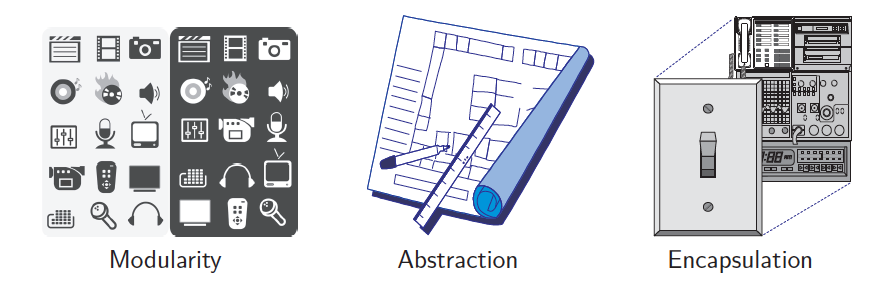
\includegraphics[width=11cm]{asp-03-pic01.png}
  \end{center}
\end{frame}

\begin{frame}[fragile]
  \frametitle{Duck typing}
  \begin{itemize}
    \item Python rukuje apstrakcijama pomoću \myred{duck typing} principa
    \begin{itemize}
      \item pesnik James Whitcomb Riley: ``when I see a bird that walks like a duck and swims like a duck and quacks like a duck, I call that bird a duck''
    \end{itemize}
  \end{itemize}
  \begin{center}
    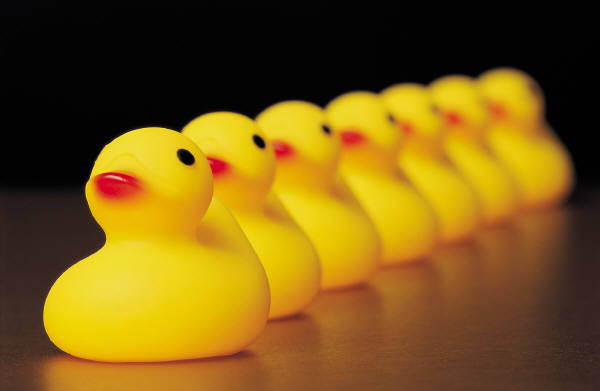
\includegraphics[width=7cm]{asp-03-pic02.png}
  \end{center}
\end{frame}

\begin{frame}[fragile]
  \frametitle{Duck typing}
  \begin{itemize}
    \item program tretira objekte kao da imaju određenu funkcionalnost ako se ponašaju ispravno i ispunjavaju traženo
    \item Python je interpretirani jezik sa dinamičkim tipovima
    \begin{itemize}
      \item nema compile-time provere tipova podataka
      \item nema posebnih formalnih zahteva kod definisanja novih tipova podataka
    \end{itemize}
  \end{itemize}
\end{frame}

\begin{frame}[fragile]
  \frametitle{Apstraktne bazne klase}
  \begin{itemize}
    \item Python radi sa ATP pomoću mehanizma \myred{apstraktnih baznih klasa} (abtract base classes, ABC)
    \item ABC se ne može instancirati, ali definiše zajedničke metode koje sve implementacije te apstrakcije moraju imati
    \item ABC se realizuje pomoću jedne ili više konkretnih klasa koje \myred{nasleđuju} ABC i implementiraju metode koje propisuje ABC
    \item možemo koristiti postojeće ABC i postojeće konkretne klase iz Python-ove biblioteke 
  \end{itemize}
\end{frame}

\begin{frame}[fragile]
  \frametitle{Enkapsulacija}
  \begin{itemize}
    \item komponente softverskog sistema ne bi trebalo da otkrivaju detalje svog unutrašnjeg funkcionisanja
    \item neki aspekti strukture podataka su \myred{javni}
    \item a neki predstavljaju interne detalje i \myred{privatni} su
    \item Python delimično podržava enkapsulaciju 
    \begin{itemize}
      \item konvencija: atributi i metode koje počinju donjom crtom (npr. \texttt{\_secret}) su privatni i ne treba ih koristiti izvan klase 
    \end{itemize}
  \end{itemize}
\end{frame}

\begin{frame}[fragile]
  \frametitle{Šabloni dizajna (design patterns)}
  \begin{tabular}{p{0.5\textwidth}p{0.4\textwidth}}
  \myred{algoritamski šabloni} & \myred{šabloni dizajna} \\ \hline
  \begin{itemize}
    \item rekurzija
    \item amortizacija
    \item podeli pa vladaj
    \item odseci pa traži
    \item gruba sila
    \item dinamičko programiranje
    \item pohlepni metodi 
  \end{itemize}
  &
  \begin{itemize}
    \item iterator
    \item adapter
    \item position
    \item composition
    \item template method
    \item locator
    \item factory method 
  \end{itemize}
  \\
  \end{tabular} 
\end{frame}

\begin{frame}[fragile]
  \frametitle{Objektno-orijentisani dizajn softvera}
  \begin{itemize}
    \item \myred{odgovornost}: podeliti posao različitim učesnicima, svako sa različitim odgovornostima
    \item \myred{nezavisnost}: definisati namenu svake klase što je moguće više nezavisno od drugih klasa
    \item \myred{ponašanje}: definisati ponašanje svake klase pažljivo i precizno, tako da posledice svake akcije budu dobro shvaćene od strane drugih klasa
  \end{itemize}
\end{frame}

\section[Klasa]{Klasa}
\begin{frame}[fragile]
  \frametitle{Objedinjeni jezik za modelovanje (UML)}
  \begin{itemize}
    \item Unified Modeling Language (\myred{UML}): (grafički) jezik za opis softverskih sistema
    \item prikaz klase na UML dijagramu ima tri celine:
    \begin{itemize}
      \item ime klase
      \item atribute
      \item metode 
    \end{itemize}
  \end{itemize}
  \begin{center}
    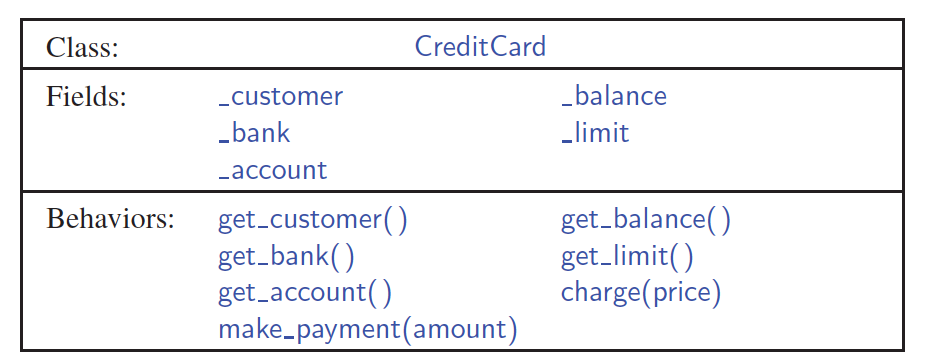
\includegraphics[width=9cm]{asp-03-pic03.png}
  \end{center}
\end{frame}

\begin{frame}[fragile]
  \frametitle{Definicije klasa}
  \begin{itemize}
    \item klasa je osnovno sredstvo apstrakcije u OOP
    \item u Pythonu je svaki podatak predstavljen instancom neke klase
    \item klasa definiše \myred{ponašanje} pomoću \textbf{metoda}; sve instance imaju iste metode
    \item klasa definiše \myred{stanje} pomoću \textbf{atributa}; svaka instanca ima svoju kopiju atributa
  \end{itemize}
\end{frame}

\begin{frame}[fragile]
  \frametitle{Identifikator \texttt{self}}
  \begin{itemize}
    \item svaka klasa može imati više svojih instanci
    \item svaka instanca ima svoj primerak atributa
    \item stanje svake instance predstavljeno je vrednošću njenih atributa
    \item \texttt{self} predstavlja instancu za koju je metoda pozvana 
  \end{itemize}
\end{frame}

\begin{frame}[fragile,shrink=10]
  \frametitle{Primer klase $_{(deo 1)}$}
\begin{minted}[linenos=false]{python}
class CreditCard:
  """Predstavlja bankarsku kreditnu karticu."""
  
  def __init__(self, customer, bank, acnt, limit):
    """Kreira novu instancu kartice.
    
    Početno stanje na računu je nula.
    
    customer  ime klijenta ('Žika Žikić')
    bank      ime banke ('ABC Banka')
    acnt      broj računa ('5931 0375 9837 5309')
    limit     ograničenje kredita
    """
    self._customer = customer
    self._bank = bank
    self._account = acnt
    self._limit = limit
    self._balance = 0
\end{minted}
\end{frame}

\begin{frame}[fragile,shrink=10]
  \frametitle{Primer klase $_{(deo 2)}$}
\begin{minted}[linenos=false]{python}
  def get_customer(self):
    """Vraća ime klijenta."""
    return self._customer

  def get_bank(self):
    """Vraća ime banke."""
    return self._bank

  def get_account(self):
    """Vraća broj računa."""
    return self._account

  def get_limit(self):
    """Vraća ograničenje kredita."""
    return self._limit

  def get_balance(self):
    """Vraća stanje računa."""
    return self._balance
\end{minted}
\end{frame}

\begin{frame}[fragile,shrink=10]
  \frametitle{Primer klase $_{(deo 3)}$}
\begin{minted}[linenos=false]{python}
  def charge(self, price):
    """Naplati datu cenu na kartice uz poštovanje limita.
    
    Vraća True ako je novac naplaćen; False ako nije.
    """
    if price + self._balance > self._limit:
      return False
    else:
      self._balance -= price
      return True

  def receive(self, amount):
    """Uplaćuje novac u datom iznosu na račun."""
    return self._balance += amount

\end{minted}
\end{frame}

\section[Posebne metode]{Posebne metode}
\begin{frame}[fragile]
  \frametitle{Konstruktori}
  \begin{itemize}
    \item kreiranje instanci klase \texttt{CreditCard}: 
  \end{itemize}
\begin{minted}[linenos=false]{python}
cc = CreditCard('Žika Žikić', 
                'ABC Banka', 
                '5931 0375 9837 5309', 
                1000)
\end{minted}
  \begin{itemize}
    \item interno će se ovo prevesti na poziv metode \texttt{\_\_init\_\_}
    \item njen zadatak je da novokreirani objekat dovede u korektno početno stanje postavljanjem odgovarajućih vrednosti atributa
  \end{itemize}
\end{frame}

\begin{frame}[fragile]
  \frametitle{Preklapanje operatora}
  \begin{itemize}
    \item eng. operator overloading
    \item ugrađene Python klase imaju definisane operatore sa prirodnom semantikom
    \item na primer, izraz \texttt{a + b} predstavlja sabiranje kod brojčanih podataka, a konkatenaciju kod stringova i lista
    \item kada pišemo svoju klasu možemo da definišemo operator \texttt{+} za instance naše klase   
  \end{itemize}
\end{frame}

\begin{frame}[fragile]
  \frametitle{Iteratori}
  \begin{itemize}
    \item iterator za bilo kakvu kolekciju podataka omogućava da se svaki element kolekcije dobije tačno jednom
    \item potrebno je napisati metodu \texttt{\_\_next\_\_} koja vraća sledeći element kolekcije 
    \item ili izaziva izuzetak \texttt{StopIteration} ako nema više elemenata \\ \\
    \item umesto \texttt{\_\_next\_\_} mogu se napraviti \\ \texttt{\_\_len\_\_} i \texttt{\_\_getitem\_\_}
  \end{itemize}
\end{frame}

\begin{frame}[fragile,shrink=15]
  \frametitle{Iteratori: primer}
\begin{minted}[linenos=false]{python}
class Range:
"""Klasa koja oponaša ugrađenu Range klasu."""

  def __init__(self, start, stop=None, step=1):
    """Inicijalizuje Range instancu."""
    if step == 0:
      raise ValueError('step cannot be 0')
    if stop is None:
      start, stop = 0, start # range(n) isto što i range(0, n)
    self._length = max(0, (stop-start+step-1)//step) # zapamti dužinu
    self._start = start # treba da zapamtimo start i step zbog __getitem__
    self._step = step

  def __len__(self):
    """Vraća broj elemenata."""
    return self._length

  def __getitem__(self, k):
    """Vraća element na poziciji k."""
    if k < 0: # za negativan k broji se od nazad
      k += len(self)
    if not 0 <= k < self.length:
      raise IndexError('index out of range')
    return self._start + k + self._step
\end{minted}
\end{frame}

\section[Nasleđivanje]{Nasleđivanje}
\begin{frame}[fragile]
  \frametitle{Nasleđivanje}
  \begin{itemize}
    \item \myred{nasleđivanje} je mehanizam za modularnu i hijerarhijsku organizaciju
    \item omogućava da se nova klasa definiše pomoću postojeće kao početne tačke
    \item postojeća klasa se obično zove \textbf{bazna}, \textbf{roditeljska} ili \texttt{super}klasa
    \item nova klasa se obično zove \textbf{potklasa}, \textbf{dete}-klasa ili \textbf{naslednik} \\ \\
    \item postoji dva načina da se potklasa učini različitom od roditelja
    \begin{itemize}
      \item potklasa može da promeni ponašanje tako što će imati novu implementaciju neke nasleđene (postojeće) metode
      \item potklasa može da proširi roditelja dodavanjem novih metoda ili atributa
    \end{itemize}
  \end{itemize}
\end{frame}

\begin{frame}[fragile]
  \frametitle{Python već koristi nasleđivanje}
  \begin{itemize}
    \item hijerarhija klasa koje predstavljaju izuzetke
  \end{itemize}
  \begin{center}
    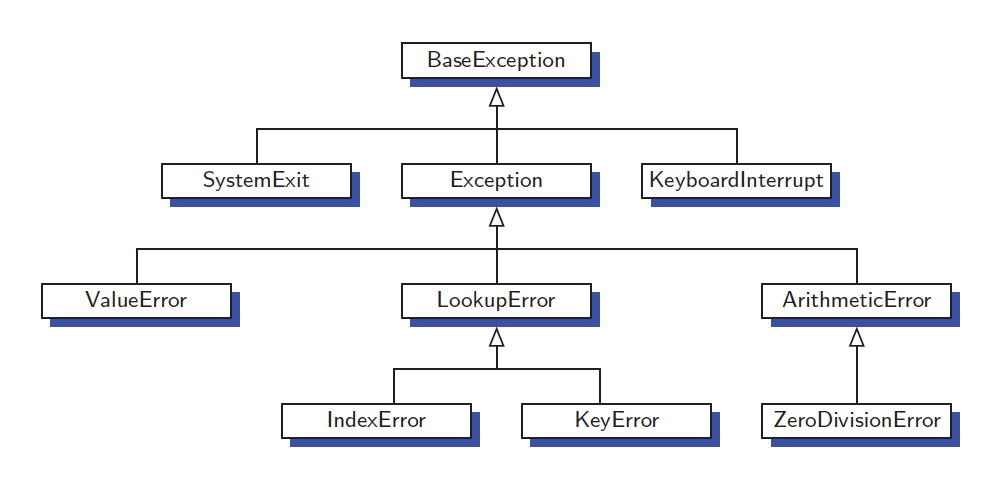
\includegraphics[width=11cm]{asp-03-pic04.png}
  \end{center}
\end{frame}

\begin{frame}[fragile]
  \frametitle{Primer 2}
  \begin{itemize}
    \item numerička progresija je niz brojeva kod koga vrednost svakog elementa zavisi od vrednosti jednog ili više prethodnih elemenata
    \item \textbf{aritmetička} progresija određuje sledeći broj dodavanjem fiksne konstante na prethodni broj
    \item \textbf{geometrijska} progresija određuje sledeći broj množenjem prethodnog broja fiksnom konstantom
    \item \textbf{Fibonačijeva} progresija koristi formulu $F_{i+1} = F_i + F_{i-1}$
  \end{itemize}
  \begin{center}
    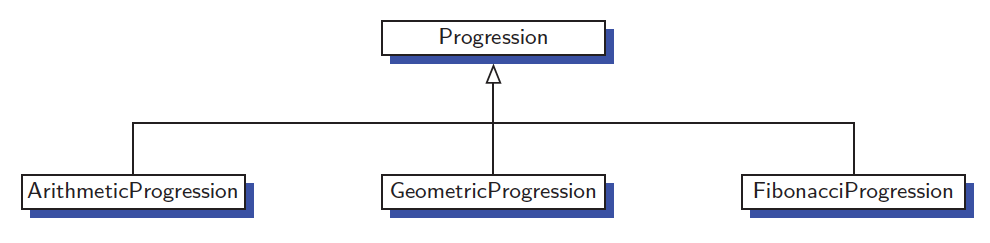
\includegraphics[width=10cm]{asp-03-pic05.png}
  \end{center}
\end{frame}

\begin{frame}[fragile,shrink=20]
  \frametitle{Primer 2: bazna klasa}
\begin{minted}[linenos=false]{python}
class Progression:
"""Iterator koji predstavlja generičku progresiju.
   Po defaultu proizvodi niz brojeva 0, 1, 2, ...
"""

  def __init__(self, start=0):
    """Inicijalizuje tekući broj na prvi broj progresije."""
    self._current = start
  
  def _advance(self):
    """Izračunava novi tekući broj self._current.
    Ovo treba da redefiniše klasa naslednica.
    Po konvenciji, None označava kraj progresije.
    """
    self._current += 1
    
  def __next__(self):
    """Vraća sledeći element ili izaziva StopIsolation izuzetak."""
    if self._current is None:
      raise StopIteration()
    else:
      answer = self._current
      self._advance()
      return answer
      
    def __iter__(self):
      """Po konvenciji iterator mora da vrati sebe kao iteratora."""
      return self
    
    def print_progression(self, n):
      """Ispisuje sledećih n vrednosti u progresiji."""
      print(' '.join(str(next(self)) for j in range(n)))
\end{minted}
\end{frame}

\begin{frame}[fragile,shrink=20]
  \frametitle{Primer 2: potklasa za aritmetičku progresiju}
\begin{minted}[linenos=false]{python}
class ArithmeticProgression(Progression): # nasleđuje Progression
"""Iterator koji proizvodi aritmetičku progresiju."""

  def __init__(self, increment=1, start=0):
    """Kreira novu aritmetičku progresiju.
       increment  fiksna konstanta koja se sabira (default je 1)
       start      prvi element progresije (default je 0)
    """
    super().__init__(start) # poziv konstruktora bazne klase
    self._increment = increment
  
  def _advance(self): # redefinišemo nasleđenu metodu
    """Izračunava novi tekući broj dodajući increment. """
    self._current += self._increment
\end{minted}
\end{frame}

\begin{frame}[fragile,shrink=20]
  \frametitle{Primer 2: potklasa za geometrijsku progresiju}
\begin{minted}[linenos=false]{python}
class GeometricProgression(Progression): # nasleđuje Progression
"""Iterator koji proizvodi geometrijsku progresiju."""

  def __init__(self, base=2, start=1):
    """Kreira novu geometrijsku progresiju.
       base       fiksna konstanta kojom se množi (default je 2)
       start      prvi element progresije (default je 1)
    """
    super().__init__(start) # poziv konstruktora bazne klase
    self._base = base
  
  def _advance(self): # redefinišemo nasleđenu metodu
    """Izračunava novi tekući broj množeći ga sa base. """
    self._current *= self._base
\end{minted}
\end{frame}

\begin{frame}[fragile,shrink=20]
  \frametitle{Primer 2: potklasa za Fibonačijevu progresiju}
\begin{minted}[linenos=false]{python}
class FibonacciProgression(Progression): # nasleđuje Progression
"""Iterator koji proizvodi Fibonačijevu progresiju."""

  def __init__(self, first=0, second=1):
    """Kreira novu Fibonačijevu progresiju.
       first      prvi element progresije (default je 0)
       second     drugi element progresije (default je 1)
    """
    super().__init__(first)   
    self._prev = second-first # izmišljena vrednost pre prve
  
  def _advance(self): # redefinišemo nasleđenu metodu
    """Izračunava novi tekući broj sabirajući prethodna dva. """
    self._prev, self._current = self._current, self._prev + self._current
\end{minted}
\end{frame}

\end{document}
